\documentclass[12pt,letterpaper]{article}

\usepackage{graphicx,wrapfig,colordvi,color,citesort,times,array,subfigure,floatflt,makeidx,framed,boxedminipage,url,hyperref}

\graphicspath{{images/}}
\definecolor{UglyBrown}{rgb}{0.7,0.4,0.1} 
\newcommand{\newtext}[1]{\textcolor{UglyBrown}{#1}}

\newcommand{\contributors}{
Thomas Parker\\
Devon Jones\\
James Dempsey\\
Aaron Divinsky\\
Tir Gwaith (Andrew McDougall)\\
Frank Kliewe\\
Eddy Anthony\\
Thomas Clegg\\
Paul W. King\\
Paul Grosse\\
Terry FitzSimons\\
Chris Chandler\\
Martijn Verburg\\
Connor Petty\\
}
\newcommand{\lastupdate}{August 8, 2008}
\newcommand{\versionEOS}{0.70}
\newcommand{\lastversionEOS}{0.60}
\newcommand{\pcgenversEOS}{5.16}

\makeindex

\hoffset=-0.6in
\voffset=-0.6in
\textwidth=6.5in
\textheight=9.0in
\parindent=0.25in
\parskip=1.0ex

\newcommand{\version}{\versionEOS{} }
\newcommand{\lastversion}{\lastversionEOS{} }
\newcommand{\pcgenvers}{\pcgenversEOS{} }

\definecolor{Red}{rgb}{1,0,0} 
\definecolor{Blue}{rgb}{0,0,1} 
\definecolor{Black}{rgb}{0,0,0} 
\newcommand{\redtext}[1]{\textcolor{Red}{#1}}
\newcommand{\revisedtext}[1]{\textcolor{Blue}{#1}}

\newcommand{\newtextPointZeroTwo}[1]{#1}
\newcommand{\revisedtextPointZeroTwo}[1]{#1}

\newcommand{\newtextPointZeroThree}[1]{#1}
\newcommand{\revisedtextPointZeroThree}[1]{#1}

\newcommand{\newtextPointZeroFour}[1]{#1}
\newcommand{\revisedtextPointZeroFour}[1]{#1}
\newcommand{\deletedTextPointZeroFour}[1]{}

\newcommand{\newtextPointZeroFive}[1]{#1}
\newcommand{\revisedtextPointZeroFive}[1]{#1}
\newcommand{\deletedTextPointZeroFive}[1]{}

\newcommand{\newtextPointTwo}[1]{#1}
\newcommand{\revisedtextPointTwo}[1]{#1}
\newcommand{\deletedTextPointTwo}[1]{}

\newcommand{\newtextPointThree}[1]{#1}
\newcommand{\revisedtextPointThree}[1]{#1}
\newcommand{\deletedTextPointThree}[1]{}

\newcommand{\newtextPointFour}[1]{#1}
\newcommand{\revisedtextPointFour}[1]{#1}
\newcommand{\deletedTextPointFour}[1]{}

\newcommand{\newtextPointFive}[1]{\newtext{#1}}
\newcommand{\revisedtextPointFive}[1]{\revisedtext{#1}}
\newcommand{\deletedTextPointFive}[1]{}

\newcommand{\textem}[1]{\emph{#1}}
\newcommand{\ix}[1]{#1\index{#1}}
\newcommand{\tool}[1]{\textbf{\ix{#1}}}

\newcommand{\rejected}[1]{}

\newcommand{\nsection}[1]{\newpage \section{#1}}
\newcommand{\lsection}[1]{\label{#1}\section{#1}}
\newcommand{\lnsection}[1]{\label{#1}\nsection{#1}}
\newcommand{\lsubsection}[1]{\label{#1}\subsection{#1}}
\newcommand{\lnsubsection}[1]{\newpage\label{#1}\subsection{#1}}
\newcommand{\lsubsubsection}[1]{\subsubsection{#1}\label{#1}}
\newcommand{\lisection}[1]{\section{#1}\label{#1}\index{#1}}
\newcommand{\lisubsection}[1]{\subsection{#1}\label{#1}\index{#1}}
\newcommand{\lisubsubsection}[1]{\lsubsubsection{#1}\label{#1}\index{#1}}

\newcommand{\myref}[1]{\ref{#1} #1}

\newcommand{\sidebar}[5]{
\noindent
\definecolor{shadecolor}{#2}{#3}
\begin{minipage}{\textwidth}
\setlength{\parskip}{-11pt}
\begin{shaded}\textbf{#1: #4}\end{shaded}
\begin{boxedminipage}{\textwidth}
#5
\end{boxedminipage}
\end{minipage}
}

\newcommand{\authors}{Members of the PCGen Development Team and Community (see contributors)}

\newcommand{\csidebar}[6]{
\noindent
\definecolor{shadecolor}{#2}{#3}
\begin{minipage}{\textwidth}
\setlength{\parskip}{-11pt}
\begin{shaded}\textbf{\textcolor{#6}{#1: #4}}\end{shaded}
\begin{boxedminipage}{\textwidth}
#5
\end{boxedminipage}
\end{minipage}
}

\newcommand{\sbdevon}[2]{\sidebar{Devon's Thoughts}{gray}{0.9}{#1}{#2}}
\newcommand{\sbjames}[2]{\sidebar{James' Thoughts}{gray}{0.9}{#1}{#2}}
\newcommand{\sbtom}[2]{\sidebar{Tom's Thoughts}{gray}{0.9}{#1}{#2}}

\newcommand{\sbnote}[2]{\sidebar{Note}{gray}{0.9}{#1}{#2}}
\newcommand{\sbwhatis}[2]{\sidebar{What Is}{gray}{0.8}{#1}{#2}}
\newcommand{\sbeffect}[2]{\sidebar{Effect}{gray}{0.8}{#1}{#2}}
\newcommand{\sbexception}[2]{\sidebar{Exception}{gray}{0.7}{#1}{#2}}
\newcommand{\sbwarning}[2]{\csidebar{Warning}{gray}{0.3}{#1}{#2}{white}}
\newcommand{\sbold}[2]{\csidebar{Original Proposal}{gray}{0.3}{#1}{#2}{white}}

\newcommand{\vbar}{\hspace{0.2mm}\rule{0.2mm}{3mm}\hspace{0.2mm}}

\newcommand{\openfig}{\begin{figure}[hbt]}
\newcommand{\closefig}[1]{\vspace*{-0.15in}\caption{#1}\end{figure}}

\newcommand{\openffig}[2]{\begin{floatingfigure}[#1]{#2}}
\newcommand{\closeffig}[1]{\caption{#1}\end{floatingfigure}}
\newcommand{\nocapcloseffig}{\end{floatingfigure}}

\newcommand{\mapffig}[4]{\openffig{#1}{#2}\includegraphics[scale=0.675]{#3}\closeffig{#4}}
\newcommand{\mapffigl}[3]{\mapffig{l}{#1}{#2}{#3}}
\newcommand{\mapffigr}[3]{\mapffig{r}{#1}{#2}{#3}}

%\newcommand{\mapfig}[2]{\openfig\centerline{\includegraphics[scale=0.675]{#1}}\closefig{#2}}
%\newcommand{\subf}[3]{\subfigure[#1]{#2\includegraphics[scale=0.675]{#3}}}
%\newcommand{\maptwofig}[7]{\openfig\begin{center}\mbox{\subf{#1}{#2}{#3}\hspace{0.25in}\subf{#4}{#5}{#6}}\end{center}\caption{#7}\end{figure}}
%\newcommand{\mapfigl}[3]{\mapfig{#2}{#3}}%\mapfig{l}{#1}{#2}{#3}}
%\newcommand{\mapfigr}[3]{\mapfig{#2}{#3}}%\mapfig{r}{#1}{#2}{#3}}
%\newcommand{\mapscalefig}[5]{\openffig{#1}{#2}\includegraphics[#3]{#4}\nocapcloseffig}

\newcommand{\mapscalefig}[3]{\openfig\centerline{\includegraphics[#1]{#2}}\closefig{#3}}
\newcommand{\mapfig}[2]{\openfig\centerline{\includegraphics[scale=0.675]{#1}}\closefig{#2}}
\newcommand{\subf}[3]{\subfigure[#1]{#2\includegraphics[scale=0.675]{#3}}}
\newcommand{\maptwofig}[7]{\openfig\begin{center}\mbox{\subf{#1}{#2}{#3}\hspace{0.25in}\subf{#4}{#5}{#6}}\end{center}\caption{#7}\end{figure}}

\newcommand{\basis}{\noindent\textem{Basis for this requirement:} }
\newcommand{\under}{\noindent\textem{Underlying Requirement(s):} }

\renewcommand{\baselinestretch}{1.0}
\hyphenpenalty=9999
\exhyphenpenalty=9999
\pagestyle{empty}
\sloppy
%\thispagestyle{empty}


%============================================================================

\begin{document}

\begin{center}

\vspace*{2.5in}
{ \Huge PCGen \pcgenvers Architecture Overview }

{ \huge Version \version (Draft) }

{ \huge Architecture Overview Document }

{ \Large Document Index Number 0.0 }

{ \large \authors }

\lastupdate

\end{center}

\vspace*{2.5in}

\noindent Portions \copyright  2006-2008 Individually by \authors.
This work is licensed under the Creative Commons Attribution-NonCommercial-ShareAlike License.
To view a copy of this license, visit \url{http://creativecommons.org/licenses/by-nc-sa/2.5/}
or send a letter to Creative Commons, 543 Howard Street, 5th Floor,
San Francisco, California, 94105, USA.

\noindent ``d20 System'' is a trademark or registered trademark 
of Wizards of the Coast, Inc., a subsidiary of Hasbro, Inc., in the United States and/or other countries.
All other trademarks mentioned are the property of their respective owners.

\newpage
\pagestyle{plain}
\setcounter{page}{1}
\pagenumbering{roman}
\tableofcontents

\listoffigures

\lnsection{Purpose and Scope of this Document}
\setcounter{page}{1}
\pagenumbering{arabic}

In 2005, the PCGen project formed an Architecture team to help define the
path forward for the software structure of PCGen.  The subsequent discussions
and architecture development led to a new proposed architecture for PCGen 6.0.

This document is a result of those efforts.  This is an interim document
leading to the transition to PCGen 6.0.  It is primarily intended to
communicate the strategic architecture of PCGen 5.16.  This document
provides a high level overview of the architecture.  Further details of
specific subsystems and processes are provided in separate documents.

\lsection{Contributors}

\newtextPointZeroThree{
Contributors to this document, either directly or by feedback and comments:\\
\contributors
}

\lnsection{Role Playing Character Generation - Background}

PCGen is a character generator for role-playing games. The project's current focus is on Open Gaming License
(OGL) games, which are generally based on systems similar to the d20 System from Wizards of the Coast. The
long-term goal of PCGen is to support as many RPGs as possible.  Support for other game systems will require
significant development, and one goal of PCGen \pcgenvers is to start a foundation from which support for additional
game systems can be developed.

\lsubsection{System Overview}

PCGen is primarily designed to allow a user to create a player character (PC) for a role-playing game. 
Specifically, PCGen supports level advancement, with configurable progressions of feats, skills, and
ability score bonuses, etc.

To faciliate the creation of a PC desired by a user, PCGen supports user modifiable data files.  This
allows support for house rules, custom combinations, and new game systems.

Once a PC is created, PCGen has flexibility to customize the PC and provide various methods of outputting
a PC from PCGen.  User modifiable Ouptut Sheets, including compatibility for PDF, HTML, XML and plain text
output are available.

PCGen also ships with numerous tools for Game Masters, as part of the GMGen plugin.

\lnsection{Functional Requirements}

The following functional requirements are provided for use in understanding the basis for the PCGen \pcgenvers 
architecture. Functional requirements are constraints on features as they appear to a user of PCGen \pcgenversEOS.

\lsubsection{Compatibility with PCGen 5.x}

PCGen \pcgenvers  must be capable of fully loading PCGen 5.14 PCC and LST data files.  Data from older 5.x releases
(in particular PCGen 5.12 and 5.10) may be compatible with PCGen \pcgenversEOS; however, there are known
ambiguities that prevent 100\% compatibility with older releases.  

This requirement must be met.  Other features of the system (requirements and other good design guidelines)
will be sacrified to meet this requirement.

\basis There is a tremendous investment in the PCGen 5.x code, data and documentation.  This compatibility
requirement ensures the ability to leverage that time investment, especally in data and documentation.

\lsubsection{Increased Flexibility}

Eliminating hardcoded values and special cases that currently exist in the PCGen code base will allow PCGen
to more easily support non-d20 systems.

\basis Expansion of the PCGen universe to include non-d20 based game systems to increase function for existing
users and to attract new users to PCGen.

\lnsection{Structural Requirements}

The following structural requirements are provided for use in understanding the basis for the PCGen \pcgenvers 
architecture.  Structural requirements constraints on features as they appear to a developer of PCGen
\pcgenversEOS.\footnote{It is recognized that some of these items would qualify more as ``design'' than 
``architecture'', as they are general features or characteristics of well written software systems. 
Without any disrespect for software architecture purists, we include a number of those design characteristics,
as they help to contrast the PCGen 5.x and \pcgenvers  architectures.}

\lsubsection{Minimize Process/Structural Models}

PCGen \pcgenvers  should have a minimal set of design structures used to specify the functions required to build a
Player Character. 

\basis This minimizes the number of mental models a developer must understand. Reduced quantity of design patterns
and structures improves the ability of new (and existing!) developers to understand the code.  This also allows
greater code reuse and reduces code duplication (which is subject to copy/paste error).  Selection of appropriate
models will also reduce the number of exceptions in the code, eliminating further risk of bugs and confusion for developers.

\lsubsection{Information Hiding}

The format of data files on disk should be independent of the processing of a game system or Player Character

\basis This insulates the code code (modifying a player character or the game system data) from changes in the
data file format.  This increases the flexibility to add features to PCGen witout core changes.  This facilitates
unit testing by improving component isolation.

\lsubsection{Data Encapsulation}

There should be defined and limited interfaces between modules of PCGen.

\basis This improves code maintainability.  This truly insulates modules of PCGen from changes elsewhere in the
system.  This therefore facilitates parallel development.  This also improves the ability to unit test the code,
as ``mock'' objects that implement the framework can be used for testing.

\lsubsection{Stable Code Structure}

Dependency between packages and classes will result in a Directed Acyclic Graph.

\basis The PCGen code base is over 1,500 classes.  This is a significant code base and requires isloating subsystems
and defining dependencies in order to minimize the impact of code changes.  Improved code structure also facilitates
testing.  Eliminating tangles in Class dependency will improve the ability to write true unit tests (tests that work
on a single Class).  This means it will be possible to catch smaller errors due to incorrect modifications of the PCGen
code base.  Improved structure also facilitates understanding of the code by developers.  The overall impact of good code
structure is seen to both developers and end users as improved speed and ability to modify the PCGen code.

For further information on why this is important, you can read the following
document:\footnote{Actually much of the series is interesting -� Tom Parker 11/18/06}
\url{http://www.objectmentor.com/resources/articles/granularity.pdf}

\lsubsection{Avoid Contracts}

Two forms of contracts should be avoided: (1) When a developer makes a code modification, the developer should not
be forced to make a matching modification in another location in the code. (2) When a change is made to the internal
data structure, a significant amount of ``reorganization'' to ensure a valid data structure should not be necessary.

\basis Contracts cause problems because they introduce bugs into software when matching changes are not made.  They also
make it more difficult for developers to understand the architecture of a system, because they are forced to focus on
adhering to the contracts.  Data structure contracts can result in invalid data structures, and often lead to performance 
issues as the data structure is validated and corrected.

\lsubsection{Minimize Order Dependency}

The number of order dependent operations should be minimized.

\basis Order dependency can cause significant issues, especially as it is hard to maintain accurate documentation of such
restrictions.  Operations which are not order dependent can also be parallelized (e.g. on multi-processor systems) to
improve performance.

\lnsection{Architecture Summary}

\lsubsection{Key Design Decisions}

\lsubsubsection{Data Persistence Interface}

The Data Persistence format must be independent of internal data structure. (The internal data structure must not have
knowledge of the data persistence file format)

\under \myref{Information Hiding}

\basis This abstracts data persistence from the internal data structure.  It forces the entire persistence contents to
be parsed on data load.  This ensures any errors in data files are caught at data load, rather than at runtime.

\lsubsubsection{The Persistence System IO}

The input and output of data persistence information should be an integral part of the data persistence system.

\under \myref{Data Encapsulation}, \myref{Information Hiding}

\basis Adding output to the persistence system provides the ability to reuse the data persistence system in a data
file editor, as well as the runtime system.  This sharing of code helps to guarantee the integrity of the data file
editor.  Such a structure also facilitates unit testing, as the persistence system can be tested independently of
the core code.

\lsubsubsection{Character Persistence Interface}

The Character Persistence format must be independent of the core code and data structure. (The internal PC data
structure must not have knowledge of the PC persistence file format)

\under \myref{Information Hiding}

\basis This abstracts character persistence from the internal data structure.  This also implies and ensures that
when a character is saved, it can be restored, even independent of the original persistent data being available.

\lsubsubsection{Catch Errors Early}

Errors in the data files should be caught during data file load, and should not trigger runtime errors.
 
\under \myref{Information Hiding}

\basis Given data persistence being independent of the internal data structure, all references will be resolved at
load time.  This will ensure that all objects in a given namespace possess a unique KEY, regardless of the source file. 
Also, all object references can be validated to ensure an object that was actually constructed and loaded.

\lsubsubsection{Shared Persistence System with Editor}

The data persistence system should be usable for both a data file editor and the runtime character generation program.

\under Code Reuse (general design characteristic)

\basis A significant investment made in ensuring that persistent data is read without errors should be reused across
both a data file editor and the runtime system.  This reduces the risk of error, ensures that the editor will always
be up to date (a problem in PCGen 5.x) and provides additional editing capabilities (e.g. edit data in place) that are
not available in PCGen 5.x.

\lsubsection{Architecture Views}

\lsubsubsection{Layered Subsystem View}

\openfig\centerline{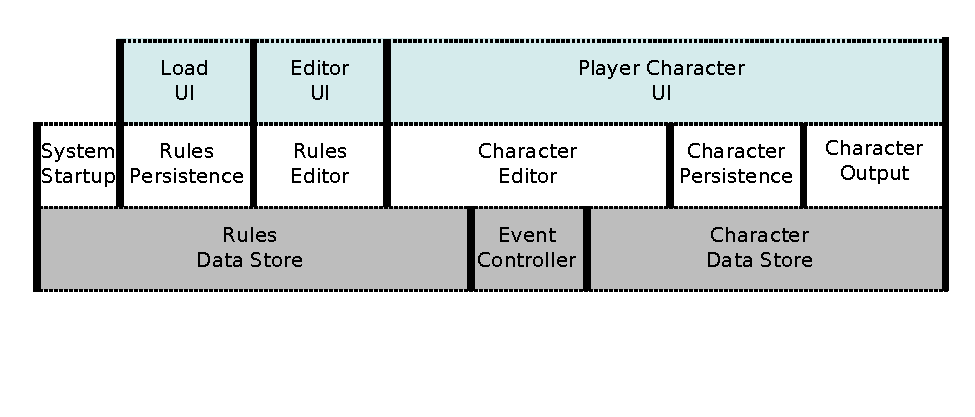
\includegraphics[width=6.5in]{osf.pdf}}\closefig{\label{Fig: Layered Subsystems}Layered View of PCGen \pcgenvers  subsystems}

\begin{tabular}{ | m{1.5in} | m{4.5in} | }
\hline
  \textbf{Element in Figure \ref{Fig: Layered Subsystems}} & \textbf{Element Description} \\  \hline \hline
  Load UI & The \textem{Load UI} is responsible for presenting the user with the options of game systems and components available to be loaded.  The LoadUI triggers a call to the \textem{Rules Persistence} system when the user requests for specific data to be loaded, and to the \textem{Character Persistence} system when the user requests for a Player Character to be loaded.. \\ \hline
  Editor UI & The \textem{Editor UI} is responsible for presenting the user with the contents of the \textem{Rules Data Store}.  It communicates requests to change the contents of the \textem{Rules Data Store} to the \textem{Rules Editor} system. \\ \hline
  Player Character UI & The \textem{Player Character UI} is responsible for presenting the user with the contents of the PC, including all of the PC's characteristics.  Requests to modify a PC are sent to the \textem{Character Editor} system for action. \\ \hline
  Startup System & The \textem{Startup System} is responsible for the activities required to load PCGen to the state where a user can select an option from the \textem{Load UI}. This includes discovery of Plugins. \\ \hline
  Rules Persistence & The \textem{Rules Persistence} system is responsible for loading game system and component data from the data file format and saving it back into that data file format. \\ \hline
  Rules Editor & The \textem{Rules Editor} system is responsible for providing the capability to modify the \textem{Rules Data Store}.  This includes modifying existing items and inserting new items into the \textem{Rules Data Store}. \\ \hline
  Character Editor & The \textem{Character Editor} system is responsible for providing the capability to modify the PC.  Changes to the PC are communicated to the \textem{Event Controller} as well as written into the \textem{Character Data Store}. \\ \hline
  Character Persistence & The \textem{Character Persistence} system is responsible for loading and saving PCs into the specified file format. Teh \textem{Character Persistence} system is also responsible for creating and initializing a new Player Character.  \\ \hline
  Character Output & The \textem{Character Output} system is responsible for resolving the active objects on a PC, searching those objects to find specific information, and preparing that information for consumption by any of the systems that desire PC information. \\ \hline
  Rules Data Store & The \textem{Rules Data Store} is the internal data structure used to store the game system and component information. \\ \hline
  Event Controller & The \textem{Event Controller} acts as a hub to communicate events (typically triggered by changes to a PC) to the UI and to any loaded Plugins.  \\ \hline
  Character Data Store & The \textem{Character Data Store} is the internal data structure used to store the PC. \\ \hline
\end{tabular}

\begin{tabular}{ | m{1.75in} | m{4.25in} | }
\hline
  \textbf{Element in Figure \ref{Fig: Layered Subsystems}} & \textbf{Subsystem Document} \\  \hline \hline
  Load UI & Subsystem Document not in scope for PCGen \pcgenvers (??) \\ \hline
  Editor UI & Subsystem Document not in scope for PCGen \pcgenvers \\ \hline
  Player Character UI & Subsystem Document not in scope for PCGen \pcgenvers \\ \hline
  Startup System & Subsystem Document not in scope for PCGen \pcgenvers (??) \\ \hline
  Rules Persistence & Subsystem Document Index 2.0 \\ \hline
  Rules Editor & Subsystem Document not in scope for PCGen \pcgenvers (??) \\ \hline
  Character Editor & Subsystem Document not in scope for PCGen \pcgenvers \\ \hline
  Character Persistence & Subsystem Document not in scope for PCGen \pcgenvers  \\ \hline
  Character Output & Subsystem Document not in scope for PCGen \pcgenvers \\ \hline
  Rules Data Store & Subsystem Document Index 1.0 \\ \hline
  Event Controller & Subsystem Document not in scope for PCGen \pcgenvers  \\ \hline
  Character Data Store & Subsystem Document not in scope for PCGen \pcgenvers \\ \hline
\end{tabular}

\lsubsubsection{Use Cases}

\openfig\centerline{\includegraphics[width=6.5in]{usecases.png}}\closefig{\label{Fig: Use Cases}Use Cases for PCGen \pcgenvers }

\begin{tabular}{ | m{1.5in} | m{4.5in} | }
\hline
  \textbf{Element in Figure \ref{Fig: Use Cases}} & \textbf{Element Description} \\  \hline \hline
  Player & The \textem{Player} is a typical user of PCGen who alters Player Characters. \\ \hline
  Game Master & The \textem{Game Master} is a user of PCGen who alters not only Player Characters, but also the underlying Rules Data. \\ \hline
  Load Rule Set & The \textem{Load Rule Set} use case occurs when a user of PCGen loads a given set of Campaigns into PCGen. More details about this use case are contained in Section \ref{Load Rule Set Collaboration View}. \\ \hline
  View Player Character & The \textem{View Player Character} use case occurs when a user of PCGen loads a Player Character (may be a new character) into PCGen for viewing.  This use case requires that the \textem{Load Rule Set} use case has already been executed. More details about this use case are contained in Section \ref{View Player Character Collaboration View}. \\ \hline
  Edit Player Character & The \textem{Edit Player Character} use case occurs when a user of PCGen changes a Player Character.  This use case requires that the \textem{View Player Character} use case has already been executed. More details about this use case are contained in Section \ref{Edit Player Character Collaboration View}. \\ \hline
  Output Player Character & The \textem{Output Player Character} use case occurs when a user of PCGen outputs a Player Character to a file (or printer).  This use case requires that the \textem{View Player Character} use case has already been executed. More details about this use case are contained in Section \ref{Output Player Character Collaboration View}. \\ \hline
  Edit Rules Data & The \textem{Edit Rules Data} use case occurs when a user of PCGen changes the rules data. This use case requires that the \textem{Load Rule Set} use case has already been executed. More details about this use case are contained in Section \ref{Edit Rules Data Collaboration View}. \\ \hline
\end{tabular}

%\newpage
%\printindex

\end{document}

